\documentclass[11pt]{scrartcl}
\usepackage{a4, fullpage}

\usepackage{color, xcolor}
\usepackage{listings, caption, graphicx}
\usepackage{multicol, titlesec}

\titleformat
	{\paragraph}
	{\normalfont\normalsize\bfseries}
	{\theparagraph}{0.5em}{}
\titlespacing*
	{\paragraph}
	{0pt}
	{1ex plus 0.5ex minus .2ex}
	{1ex plus .2ex}

\renewcommand{\lstlistingname}{Snippet}

\DeclareGraphicsExtensions{.pdf,.png,.jpg}
\DeclareCaptionFont{white}{\color{white}}
\DeclareCaptionFormat{myformat}{#1#2#3\hrulefill}

\captionsetup{format=myformat}
\captionsetup[lstlisting]{
	position = bottom,
	format = myformat
}

\lstloadlanguages{ruby}
\lstset{
	basicstyle   = \ttfamily\color{black},
	commentstyle = \ttfamily\color{red},
	keywordstyle = \ttfamily\color{blue},
	stringstyle  = \color{orange}
}

\setlength{\parskip}{0.4cm}
\setlength{\parindent}{0cm}

\begin{document}

\title{Musical Concurrent Programming \\ With Sonic Pi}
\subtitle{Interim Report}
\author{Eleanor Vincent}
\date{\today}
\maketitle

\section{Introduction}

\subsection{Motivation}
For many years it has not been a requirement that children should learn much
about the vast field of computing during their formative years in UK 
Education. Some of the earliest significant pieces of work towards the 
education of computing started with the invention of Logo, an adaptation of 
the LISP language, most remembered for its use of ``turle graphics''. Some 
time after this came the Computers in the Cirriculum Project, funded from 
1972 to 1991 by the Schools Council and subsequently by the Microelectronics 
Education Programme in 1981. The first microcomputers appeared in both UK 
Primary and Secondary Schools in 1979. The Commodore Pets aided both spelling 
and arthimetic practice as well as the ability to teach either BASIC or Logo. 
The 1980's saw a huge amount of legislative reform and technical efforts in the 
vein of giving young people the ability to work with computers during their 
formative years but over the course of the late 80's and early 90's this focus 
on programming ability gives way to simply the education of practical use of 
existing computer software instead of a focus on the fundamentals behind these 
applications \cite{naec}.

In 2013, Ofsted published a report documenting their findings relating to ICT 
in UK schools from 2008 to 2011 and found that in half of all secondary 
schools, school leavers had not been given adequete education to move into a 
technical career in their future. In 2007, 81,100 pupils were enrolled in the 
ICT GCSE but this had fallen to 31,800 pupils by 2011 \cite{DfEO13} with a 
notable lack in the education of key skills such as computer programming 
itself. This lack was found to be as much a lack in knowledge from the 
teacher's as much as the cirriculum's failure to address the issues.

In 2012, the Government began to recog the signifiance of Computer Science and 
has replaced the National ICT curriculum with a revised Computing cirruculum. 
The new Computing Program of Study \cite{DfE13} aims to enable pupils to 
understand the world of computing, giving them the ability to think logically 
and apply the fundamental principles of the discpline to their real-world 
environments.

Along a similar vein there is a general struggle within the humanties courses 
available in schools to remain relevant in light of a quickly developing 
technical world. Music schemes within the UK frequently report to have 
suffered funding cuts and education is focused on learning a variety of 
specific instruments, with little focus on musical technology until the later 
years of education.

As well as the necessity of Computer Science and Music within schools, there 
is an increasing recognition of the power of programming amongst the general 
populace. A growing hacker and maker movement has been making programming a 
much more accessible skill \cite{BAD14}; it presents itself as a viable and 
useful hobby amongst a vast range of ages and professions and this is as much 
because of the availability of useful resources that would be frequently used 
in such situations as a school classroom. There is existing research that has 
gone into the viability of programming tools for professional artists, as 
reported at PPIG \cite{Ch12,BC05}, and investigations into the craft practices 
of existing professional software developers who work in professional art 
contexts \cite{W10}.

The movement is not purely restriced to the UK. In the US there is a similarly 
led campaign calling to recognise the topic as relevant to all contempary 
sciences. It calls ``Computational Thinking'' a universally applicable 
attitude and skill set everyone, not just computer scientists, would be eager 
to learn and use \cite{Wing06}.

Sonic Pi is one of many projects designed to support both computing and music 
lessons within schools. Sonic Pi is an environment for creating live-coded 
music at a level of complexity which is well suited to a first-programming 
language \cite{sp}. There are many languages in existence which are simply 
enough to also constitute as a good first-programming language, but many do 
not attempt to make themselves an inviting gateway into the realm of technical 
programming. Sonic Pi seeks to provide an exploratory and invigorating 
introduction into programming whilst being complex enough to lead a user 
through into much more complicated programming ideas and use cases with a 
managable learning curve. By presenting a musical system it seeks to break 
down the barrier between the technical elite and the hobbyist. In this report 
Sonic Pi will be presented in terms of the formalisation of its timing effects 
and the existing concurrency primitives of the language.

\subsection{Objectives}
This project's aim is to formalise the concurrency and timing aspects of the 
language and develop a program analysis tool that can be used to identify 
program bugs such as deadlock and thrashing behaviour. The formalism and 
analysis will build on initial work describing timing and concurrent 
interaction via effect systems and session types. The project combines 
theoretical aspects of type system and analysis design, as well as practical 
work developing a responsive program analysis engine.

\subsection{Report Structure}
The remainder of this report is broken down as follows:

\begin{itemize}
	\item Background: We detail the histories of Sonic Pi, Live Programming 
	and Session Types as fields of research and conclude with work relating to
	these subjects.

	\item Going Forward: The bulk of this section details the expected 
	timeline of the project and ideas for how to evaluate progress during and 
	at the conclusion of the project.
\end{itemize}
\newpage

\section{Background}
In this section we begin by explaining the ideas and features of Sonic Pi, 
the living coding program that forms the basis of this project. We then 
move on to explain the subject of both Living Programming and Session Types
in further detail and seek to relate them back to the current aims of the
project. We conclude with details on the related work in these areas of
research.

\subsection{Sonic Pi}
Sonic Pi is an imperative live programming language designed as an educational 
first language. It is a ruby-based domain-specific language designed for 
manipulation of synthesisers through time \cite{AB13}. It is currently in its 
second iteration, with the main extension between the two languages being the 
work done to improve the timing system of the project, which is discussed in 
more detail below. Sonic Pi is built on top of the SuperCollider synthesis 
server to enable it to define and manipulate synthesisers in real time; an 
important feature for a musical language. Some of the concepts that Sonic Pi 
is well suited to teach, in direct relevance to the current UK Computing in 
Schools Cirruculum, are conditionals, iteration, variables, functions, 
algorithms and data structures. Sonic Pi also extends beyond these concepts to 
include such things as multi-threading and hot-swapping of code as these are 
likely to be of crucial importance in the future of programming contexts \cite{
AOB14}.

This section first gives a breif description of the Raspberry Pi then explores 
the implementation of Sonic Pi V1.0, mainly to give appropriate context to the 
timing effects system that Sonic Pi V2.0 currently imeplments. There is then 
be some short discussion on the particular features of Sonic Pi V2.0.

\subsubsection{Raspberry Pi}
The Raspberry Pi was developed as a very low cost computer system to enable 
technical experimentation amongst young people who had little other contact 
with computer systems. The idea came about in 2006 as an answer to the 
steadily decreasing levels of pupils applying to take up Computer Science 
after their A-Levels. The reasons for this were attributed to many 
contributing events such as the end of the dot come boom, the focus of IT 
lessons on Microsoft software and building very basic HTML websites and the 
increased availability of out-of-the-box games consoles over the Amigos, BBC 
Micro, Spectrum ZX and Commodore 64 machines that promoted individual 
experimentation so freely in the past \cite{rp}.

The Pi is provided as a bare circuit board costing roughly \$25, able to boot 
into a Linux environment with very little other commerical equipment required. 
The Raspberry Pi Foundation is a non-profit organisation and has sold over a 
million products since 2012. The main objective is to develop genuine 
technical competency by allowing the freedom to experiment with the whole 
system rather than taking the locked box approach of other systems. Learning 
becomes self directed for pleasure rather than at the behest of a mark molded 
system. It is this style of engagement that brought the Raspberry Pi to the 
attention of educational campaigners and has since enabled it to be used so 
successfully within the new movement towards better Computing education within 
Schools. 

\subsubsection{Sonic Pi V1.0}
The initial development time given to Sonic Pi v1.0 was roughly three weeks. 
It was designed largely as a port from the language Overture to focus on 
driving specific educational objectives with the idea in mind to teach a 
target audience of 12-year-olds that had no previous experience with 
programming; it would bring them from the introduction of a computer through 
to the ability to write a full length program over the course of a few weeks. 
Sonic Pi was built as a ruby-based language both through the author's existing 
experience with the language and also to keep it in line with languages 
already used within the industry. Python is well regarded as an educational 
language and given the semantic similarity between Python and Ruby it was easy 
to defend Ruby as a choice of language implementation \cite{AB13}. 

The immediate feature that Sonic Pi focuses on is sequential ordering in 
imperative programs; demonstrated in musical theory by the sequential playing 
of notes. 

\begin{multicols}{2}
The Code Snippets shown demonstrate two small Sonic Pi programs. The first 
demonstates the situation where the MIDI notes would be played together. Sonic 
Pi v1.0 takes advantage of fast clockspeeds of modern processors in order to 
assume the sequence of instructions would be likely to execute quickly enough 
to sounds together. In order to separate them into sequential notes they must 
be separated with a sleep instruction as demonstrated by the second code 
Snippet. The notation for sleep in Sonic Pi V1.0 is similar to that of the 
POSIX sleep operation\cite{IG13}. The default sound that Sonic Pi uses in 
these contexts is a pleasant bell sound from the SuperCollider synthesiers.

\begin{minipage}{0.5\textwidth}
	\begin{minipage}[t]{\textwidth}
		\begin{lstlisting}[language = ruby]
	play 60
	play 61
	play 62
		\end{lstlisting}
		\captionof{lstlisting}{Chord Form: Successive Notes}
	\end{minipage}
	\begin{minipage}[t]{\textwidth}
		\begin{lstlisting}[language = ruby]
	play 60
	sleep 0.5
	play 61
	sleep 0.5
	play 62
		\end{lstlisting}
		\captionof{lstlisting}{Arpeggio Form: Sleep Separation}
	\end{minipage}
\end{minipage}

\end{multicols}

The monadic structure of the statements may not be necessarily elegant to many 
experienced programmers. However, it can be seen that the ability to skip the 
arguably verbose nature of structured syntax makes it much more relevant in 
the contexts of a classroom as pupils are able to start creating meaningful 
programs with much more speed. From the point of view of providing any future 
debugging interfaces, it has a small benefit in removing the code overhead for 
finding and correcting such small syntactical issue such as missing \texttt{;}. 

These semantics work well in an educational context but do not allow for the 
correct timing of musical notation which puts them at odds with user 
expectations. To demonstrate this more concretely, below are two further code 
Snippets demonstrating Sonic Pi's basic threading abilities. Sampling is a 
feature of Sonic Pi V2.0 but are presented here in the context of V1.0 
programs as the two versions are semantically similar.

\begin{multicols}{2}
In Snippet 3 the desired outcome is to play MIDI note 60 together with the 
drum kick with an interval of 0.5s between each hit. Unfortunately, this does 
not take into account the execution time of each statement; there is a short 
amount of execution time for each line of code, plus the desired sleep of 0.5s.
Because of this the rhythm will gradually shift with each loop as the 
clock time and the ``virtual time'' becomes further out of sync. The 
actually length of time each line execution takes is variable between 
processors depending on their speed and overall load. Regardless, we can see 
that each loop in Snippet 3 will actually take longer than the desired 0.5s.

This is further apparent when running Snippet 4. The desired outcome is to 
play the drum kick every second and the MIDI 60 note at every half second, so 
the two notes will play at the same time every second MIDI note, the threads 
remain synchronised. On running the threads it is quickly apparent that this 
is not the true result; due to differing execution times the thread rhythms 
drift apart very quickly.

	\begin{minipage}{0.5\textwidth}

		\begin{minipage}{\textwidth}
			\begin{lstlisting}[language = ruby]
loop do
    play 60
    sample :drum_heavy_kick
    sleep 0.5
end
			\end{lstlisting}
			\captionof{lstlisting}{Repeating Bass and Drum}
		\end{minipage}

		\begin{minipage}{\textwidth}
			\begin{lstlisting}[language = ruby]
in_thread
    loop do
        play 60
        sleep 0.5
    end
end

in_thread
    loop do
        sample :drum_heavy_kick
        sleep 1
    end
end
			\end{lstlisting}
			\captionof{lstlisting}{Concurrent Threads}
		\end{minipage}

	\end{minipage}

\end{multicols}

The $play$ and $sample$ calls are asynchronous and this compounds the present 
timing issue due to additional costs in sending and interpreting the messages. 
These issues are summarised in Figure 1. The left-most column represents the 
real computation time of the statement whilst the right-most column shows the 
point at which each statement would be run. Each statement duration is unique 
as processor speed and system load variations affect the duration of each 
statement separately. The durations are therefor non-deterministic in nature 
and also not consistent across different runs of the same program.

\begin{figure}[ht]
	\centering
	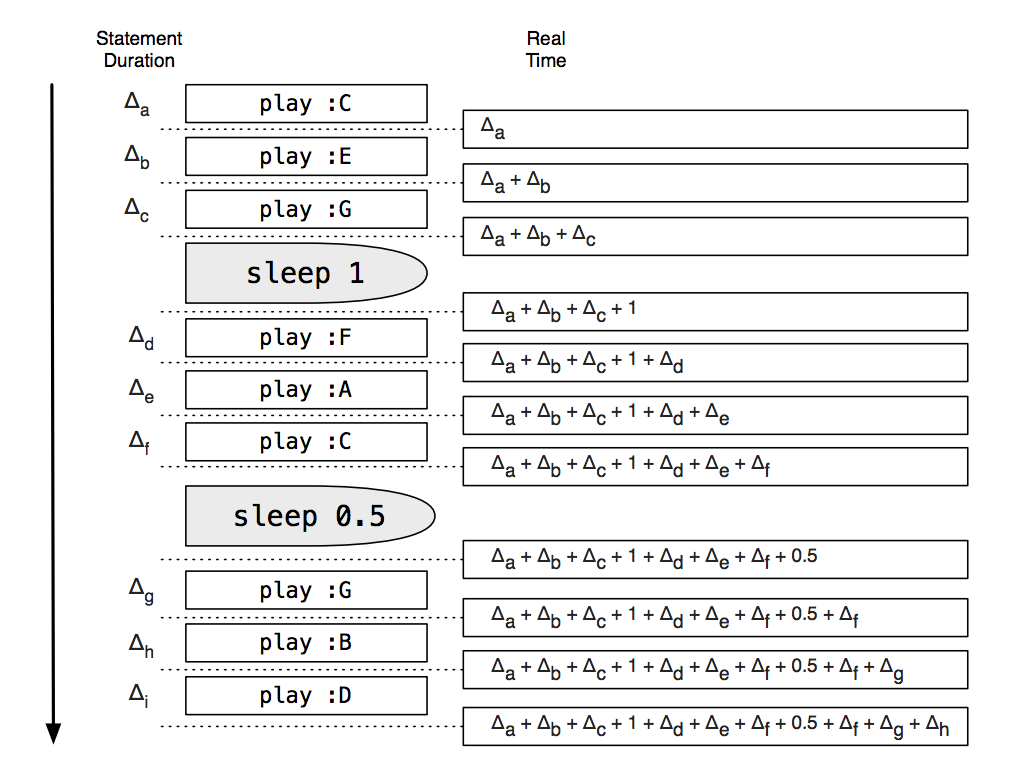
\includegraphics[width=0.9\textwidth]{images/sonic-one.png}
	\caption{Timing in Sonic Pi V1.0}
\end{figure}


\subsubsection{Sonic Pi V2.0}

\paragraph{Timing Sleep}
Sonic Pi V2.0 sought to address this temporal issue and introduces the 
interesting concept of a \emph{time system} and associated \emph{time safety}, 
which draw an analogy from the familiar programming concepts of \emph{type 
systems} and \emph{type safety}. As noted before, V2.0 maintains syntactic 
compatability with V1.0, so it conceptually as useful to apply in the 
educational context as before. The power behind V2.0 is that its temporal 
semantics now react as a user would expect them to, making it a viable program 
for the musically experienced who have some concept of what they want to 
achieve as well as for those beginners who desire to learn.

In Sonic Pi V2.0 the sleep command no longer mimics the POSIX command as 
commented earlier. Instead the programming model allows a separation of the 
ordering of effects from the timing of effects. Snippet 5 shows a simple 
example that combines the different kind of effects; parallel, timed and 
ordered effects. It also demonstrates further syntactic abilities of V2.0 as 
we are now treating the code snippets as V2.0 programs.

\begin{minipage}{\textwidth}
	\begin{lstlisting}[language = ruby]
		  play :C ; play :E ; play :G
		  sleep 1
		  play :F ; play :A ; play :C
		  sleep 0.5
		  play :G ; play :B ; play :D
	\end{lstlisting}
	\captionof{lstlisting}{V2.0 Program: Playing three chords (C major, F major, G major)}
\end{minipage}

Each chord line demonstrates Sonic Pi's ability to play notes in parallel, the 
system still taking advantage of the capabilities of modern processors. \texttt
{sleep} now acts as a ``temporal barrier'' between statements; it works by 
clocking computation from proceeding until the given time has elapsed \emph{
since the program began running}. It does \emph{not} block from the end of the 
notes played. In terms of Snippet 5, this means that the second chord is 
played once one second has elapsed and the third chord will not be played 
until 1.5 seconds have elapsed. One can think of \texttt{sleep} as an ``at 
least'' timing. In other words, once \texttt{sleep t} has been evaluated, we 
can state that at least \texttt{t} seconds have elapsed since the last \texttt{
sleep} statement was called. This is similar to how the language ChucK handles 
the interaction of time using its (multiply) overloaded \texttt{=>} operator 
\cite{WC03}.

For completeness it was worth noting that Snippet 5 demonstrates the ordered 
effect as the three chords are played in the order written.

\begin{figure}[ht]
	\centering
	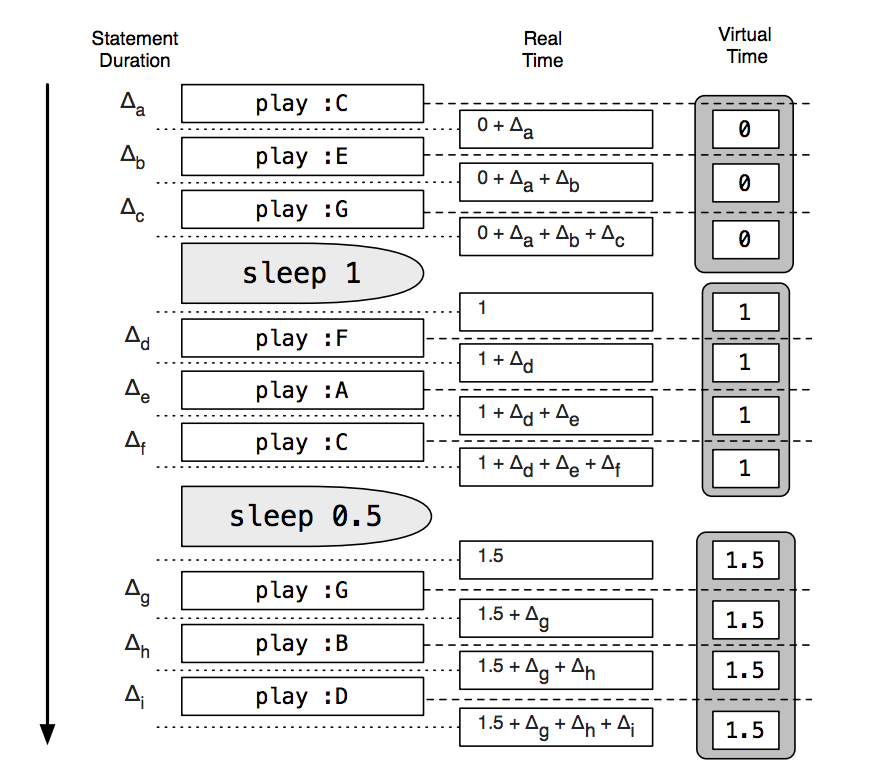
\includegraphics[width=0.8\textwidth]{images/sonic-two.png}
	\caption{Timing in Sonic Pi V2.0}
\end{figure}

The semantics introduced here are achieved by implementing a previously 
mentioned concept of ``virtual time''. In Sonic Pi V2.0, virtual time is a 
thread-local variable that is only advanced by a new \texttt{sleep} command, 
which means that the programmer has explicit control over the timing of the 
program. Each thread maintains access to both the real time elapsed and the 
virtual time elapsed whilst running a given program and used the virtual time 
variable to scheduled requested effects. In order to keep time with the 
explicit timing requirements of the program the \texttt{sleep} command will 
take account of the execution time between the last \texttt{sleep} statement 
and the current execution point. Referring back to Snippet 5, at the point at 
which the program executes the second \texttt{sleep} command, if if execution 
of the F major chord took 0.1s of execution time then the program will only 
sleep for 0.4s. This is to ensure there is no rhythm drift. The only overhead 
in the rhythm are from the play statements following the last \texttt{sleep} 
executed. This is demonstrated visiually with Figure 2.

To deal with the non-deterministic execution times within a sleep barrier, and 
also to deal with the time cost for the synthesiser to schedule output 
effects, a constant \texttt{scheduleAheadTime} value is added to the current 
virtual time for all asynchronously scheduled effects. If the jitter time and 
execution time between \texttt{sleep} commands never exceeds this value then 
the temporal requirements of Sonic Pi are met. 

It is possible that the time between \texttt{sleep} commands may over-run - 
this may be common in the event someone requested a short \texttt{sleep} time 
such as 0.1s or even 0.05s. In this case, the described programming model is 
not useful for providing hard deadlines but can function with ``soft'' 
deadlines (along the vein of Hansson and Jonsson \cite{HJ94}. In the event a 
thread falls behind in execution time then the user is given explicit 
warnings. Should the amount of time the thread is behind exceed a specific fall
-behind value, as defined within Sonic Pi, then the system will stop that 
thread and throw a time exception. This provides essential temporal 
information about the program and its behaviour to the users. This is a 
positive in terms of educational use but is something a live coder will aim to 
avoid during a real performance. This feature also provides a safety mechanism 
against common errors such as placing isolated \texttt{play} calls between \
texttt{sleep} commands which would have the problem of taking up all of the 
system resources; instead the thread self-termininates and allows any other 
threads to continue executing.

\paragraph{Threading}

Threading has already been introduced breifly; this section focuses on the 
further improvement that Sonic Pi V2.0 brings to its threading primitive. 
Within V2.0 there are multiple commands which allow for easy synchronisation 
of threads whilst the programming is running. Threads also implement thread-
based inheritance wherein they take all of the synthiser settings of the 
thread they were spawned from.

The keyword \texttt{in\_thread} is enables Sonic Pi users to run pieces of 
code concurrently. Threads can be named as shown in Snippet 6 in a similar way 
to how functions are named in Sonic Pi. The simple nature of its loop syntax 
enables this to be as easy a concept to grasp as the previously defined 
temporal semantics. These threads alone do not allow for the live coding that 
Sonic Pi has been created for. With a simple \texttt{in\_thread} it is more 
verbose to change the program sound as the program is running. For this, Sonic 
Pi V2.0 provides a \texttt{live\_loop} functionality.

An interesting point to note about Sonic Pi V2.0 is that actually running the 
program starts the current program in another thread. Because of this one can 
actually press run multiple times and have the program layered over the top of 
itself. There are no particular synchronisation primitivs defined over these 
``global'' threads, but it makes for an interesting performance if timed 
correctly.

\begin{minipage}{\textwidth}
	\begin{lstlisting}[language = ruby]
    in_thread(name: :bass) do
        loop do
          use_synth :prophet
          play chord(:e2, :m7).choose, release: 0.6
          sleep 0.5
        end
    end

    in_thread(name: :drums) do
        loop do
          sample :elec_snare
          sleep 1
        end
    end
	\end{lstlisting}
	\captionof{lstlisting}{Named Threads}
\end{minipage}

\texttt{live\_loops} can be named much more cleanly than \texttt{in\_threads} 
and are where Sonic Pi really comes into it's live coding roots. Whilst 
running a program, Sonic Pi's \texttt{live\_loops} will automatically update 
the program without skipping any beats. This gives the users a great amount of 
freedom to experiment with different sounds without having to stop the program 
and wait for anything to compile and run, as is the case with standard 
programming. This feature, however, is directly affected by the previously 
described temporal semantics, in that loops can easily become out of time with 
each other while a performance is happening. To combat this, Sonic Pi provides 
synchronisation semantics in the form of the \texttt{cue} and \texttt{sync} 
commands. Each time a live loop loops it will generate a new \texttt{cue} 
event which we are able to \texttt{sync} on to. 

\begin{minipage}{\textwidth}
	\begin{lstlisting}[language = ruby]
    live_loop :foo do
        play :c1, release: 8, cutoff: rrand(70, 130)
        sleep 8
    end
	\end{lstlisting}
	\captionof{lstlisting}{Live Loops}
\end{minipage}

\clearpage
\begin{multicols}{2}
The Snippets to the right demonstrate a rough workflow of how a user would use 
the \texttt{cue} and \texttt{sync} features. To begin with the loops 
\texttt{foo} and \texttt{bar} are out of time with one another.

To work with the current example one would begin to fix the situation by 
changing the sleep time in \texttt{foo} to 0.5s. Most likely, this will still 
sound incorrect. This is because the two loops are likely to now be out of 
time with each other. Both \texttt{foo} and \texttt{bar} are producing \texttt{
cue} events, but these are not being used and so both loops are running with 
no regard to the other. We can fix this by \emph{syncing} one thread to the 
other, so that it will only fire when the other thread has looped. In this 
case we have synced \texttt{bar} onto \texttt{foo}.

This gives way to some very obvious deadlock scenario's that users must avoid. 
If you create two live loops, \texttt{one} and \texttt{two} writing a 
situation that results in either \texttt{cue :one} in the second thread and 
\texttt{cue :two} in the first, or similar with \texttt{sync} then this will 
result in a deadlock as both threads wait for the call from the other.
	\begin{minipage}{0.5\textwidth}

		\begin{minipage}{\textwidth}
			\begin{lstlisting}[language = ruby]
live_loop :foo do
    play :e4, release: 0.5
    sleep 0.4
end

live_loop :bar do
    sample :bd_haus
    sleep 1
end
			\end{lstlisting}
			\captionof{lstlisting}{Out of Sync Live Loops}
		\end{minipage}

		\begin{minipage}{\textwidth}
			\begin{lstlisting}[language = ruby]
live_loop :foo do
    play :e4, release: 0.5
    sleep 0.5
end

live_loop :bar do
    sync :foo
    sample :bd_haus
    sleep 1
end
			\end{lstlisting}
			\captionof{lstlisting}{Synced Live Loops}
		\end{minipage}

	\end{minipage}
\end{multicols}

\paragraph{The IDE}
The IDE is as much a part of the educational experience as the language 
itself. Sonic Pi features a bespoke environment that contains only the bare 
minimum features required to enable pupils to start coding quickly and with 
minmal confusion. For this reason the IDE only consists of five key components:

\begin{itemize}
	\item Control Buttons
	\item Workspace Tabs
	\item Editor Pane
	\item Information Pane
	\item Error Pane
\end{itemize}

\begin{figure}[ht]
	\centering
	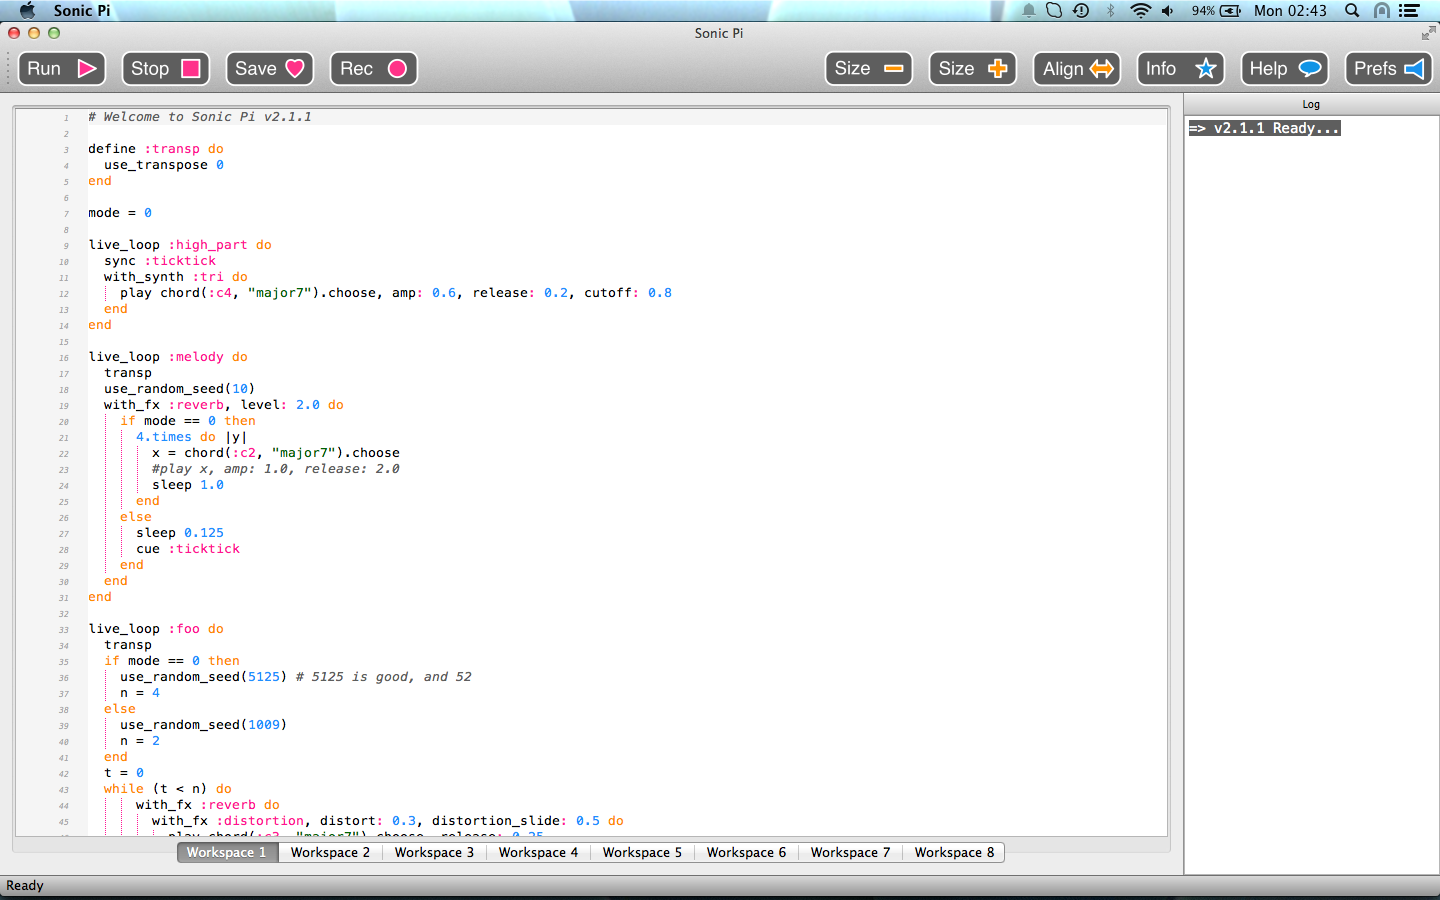
\includegraphics[width=\textwidth]{images/sonic-ide.png}
	\caption{Sonic Pi V2.1.1 IDE - Apple Mac View}
\end{figure}

Sonic Pi originally choose not to have a file save system as the workspaces 
automatically save the current session. There were no other usual IDE features 
such as project structure, macro system, refactoring wizard, etc... This is to 
keep the system as simple as possible to make it quick for young pupils and non
-IT teachers to get to grasps with.

Since then, in Sonic Pi V2.1.1, it has added the ability to save the current 
workspace to your file system, the ability to record what is playing and save 
as a .wav file type, basic formatting buttons, the ability to import other 
music files as custom samples, information and tutorial sections, all whilst 
remainind simplistic and easily useable. Features are non-intrusive but 
incredibly useful in terms of allowing those pupils who thrive with the system 
to continue to experiment outside the scope of the regular cirruculum lessons.

\subsection{Live Programming}
For much of the prevailing history of programming there has been an idea that 
the programmer is inherently separated from the system that they are 
producing. The task of the programmer is to create a system based on some 
formal specification that will take effect at some unknown point in the 
future, and the time between implementation and action has no effect on the 
results that the system will produce. In this way, there is a strong sense of 
separation between the program, process and task domains where the progam is 
the code implementation and specifications, the process is the running of the 
code on a specific machine and the task is the visible real world results
\cite{SG10}. This is a viewpoint that many would not think to challenge as it 
is natural to assume that the methodology of a computer programmer would 
naturally lend itself to implementation of actions that were set for execution 
in the future and, in general, would process a deterministic set of results 
that can be repeatedly used as the users required.

Live programming (also referred to as With Time Programming or Just In Time 
Programming) seeks to apply the improvisional nature of time to the existing 
methodology of the programmer. With this idea it becomes possible to define a 
tigher system of feedback between the program and task domains through means 
of whatever process domain is most suitable. The improvisional nature of the 
acitity also removes the inherent requirement of a specific program 
specification and allows for new level of freedom and creativity in the 
programs being created. 

Given the nature of Live Programming the languages that invoke it are often 
dynamic language which allow for the flexibility, conciseness and ease of 
development \cite{McD07} to enable the act of live programming to feel as 
natural as standard programming practice.

Live Programming lends itself also to acts of performance, where Live Coders 
will often perform to live audiences, often producing such things as live 
improvisational music or artwork, whilst having some means by which the 
audience will also see the code written at the same time. For a Live Coder 
there is frequently no desire to create a final software product or even a set 
musical score as live programming is about the experimentation rather than the 
manufacture. From a social and cultural viewpoint, Live Programming lends 
itself to breaking down the barriers that have been built up between software 
technology and the creative users \cite{McL13}.

It is interesting that the users level as a musician will have specific 
impacts on their experience with the systems in use in the context of live 
programming and audio languages. Musical scores will provide an implicit time 
representation whilst most musical languages will use explicit temporal 
structures. This generally makes the representation of rhythm within the 
language guarantee only the ordering of the notes and not the time elapsed 
between playing each one. In terms of musical experience, non-experienced 
users may be able to identify an odd sound within this system but be unable to 
pinpoint exactly what causes the problem. 

The question of time and temporal semantics within computing has been in 
existence for some time, but live programming as a field is a very young 
research area, with most of the popular languages appearing over the last 
decade. This comes as part of a wider movement of programming reaching more of 
the general populace and as it is applied with more and more creative outlets 
in mind, this separate way of thinking about the programming environment is 
likely to produce more interesting projects as time develops. Lee et al. \cite{LDW87} proposed six features that would be required to exist in order to present a programming environment with a ``first class'' semantics for time:

\begin{itemize}
	\item The ability to express timing constraints
	\item Timed communication
	\item Enforcement of timing constraints
	\item Tolerance to violations and constraints
	\item Maintaining consistency in distributed realtime systems
	\item Static timing verification
\end{itemize}

On the conclucion of the project we will seek to see how well the extended Sonic Pi application is able to address these issues, to see if it may be described as having a ``first class'' semantics.

\subsection{Session Types}
Over recent years there has been a massive increase in the amount of 
communication based systems, from network protocols over the Internet to server
-client systems in local area networks to distributed applications on a global 
scale. The crucial observation amongst all of these systems is that while 
there may be some way to describe a one-time interaction between processes 
there is no real construct to structure a series of reciprocal interactions 
between two parties \cite{HVM98}.

Session Types present a solution to the issue of structing communication-based 
software. In a similar way to how Object Oriented paradigms sought to solve 
the issues presented by large scale system written largely with spaghetti 
code, Session Types seek to restructure existing complex behaviours in a 
manner which is more lucid, readible and ultimately more easy to verify. Honda 
et al (98) present this in terms of simple concurrent primitives that build up 
a basic structuring method for communication-based concurrent programming. In 
terms of this project, we seek to use some of the binary notions of the 
project to help with the verification of communication between live threads to 
ensure safety during a system's performance. This is a very basic system to 
apply the concept to but given the inherently dynamic and concurrent nature of 
the program it presents itself as an interesting avenue of application. The 
use of Session Types in terms of Sonic Pi will be the type discipline that 
plays a fundamental role in guaranteeing the compatability of process 
interaction - it is especially effective at detecting deadlocks in a system, 
one of the primary sources of error in concurrent systems. Session Types are 
also designed in a language agnostic manner, meaning it will be possible to 
apply to Sonic Pi's Ruby-like syntax.

Session Types consist of the following key ideas:

A basic structural concept known as \emph{sessions}. These are designated via 
\emph{channels}. The collection of session interactions is what constitutes a 
program; those interactions are performed via the channels. As well as the 
session, other concurrent programming contructs are provided: parallel 
composition, name hiding, conditional and recursion. The combination of 
recursion and sessions allow for the expression of unbounded thread of 
interaction as a single abstraction unit.

Three basic communication primitives that all other structures will be built 
from: \emph{value passing} - standard synchronised message-passing, \emph{
label branching} - purified method invocation, devoid of value passing - and \
emph{delgation} - the passing of a channel to another process. Alongside 
sessions, these allow for complex structures to be defined and described with 
clarity.

Finally there is a basic type discipline for the communication primitives. 
Without this there would be no way to guarantee the typability of a program, 
ensuring that two communicating processes always have compatible patterns of 
communication. It is the incompatibility of interaction patterns that is one 
of the main reasons for bugs in commmunication-based programming.

\subsection{Related Work}
This section discusses much of the work discovered during the intial research 
of the project. There are many interesting live programming environments out 
in use in the world, with each having an interesting approach to the technical 
challenges surrounding the issue of temporal semantics. We breifly discuss 
some programs that have made use of the Session Types structures as described 
previously as this gives a clearer picture of their use and viability within 
the real world. It is worth noting that, to date, there is no apparent system 
which seeks to apply the Session Typing structure to a live programming 
paradigm to address some of the concurrency issues faced in that field.

As noted by Rorhruber \cite{BMNR14}, there have been many publications and 
discussions relating to alternative approaches for temporal semantics and 
timing within Live Programming. There is much to be said about choosing 
between explicit and implicit representation of time as well as between the 
description of time using either internal or external state.

The Tidal language \cite{McL13} uses an interesting formalisation of cyclic 
time. Whilst drawing a continuing analogy with the act of knitting, McLean 
describes the DSL for musical pattern embedded in the pure functional language 
Haskell. Tidal represents music as a pure function, enabling the mapping of 
the single dimension of time into multidimensional music, making full use of 
iterative language to formalise cyclic time using both analogue and digital 
pattern.

Impromptu is a much fuller system, able to produce both audio and visual 
outputs in the context of Live Programming \cite{SG10}. It uses ``temporal 
recursion'' as a style of time-driven, discrete-event concurrency with real-
time interrupt scheduling. This recursion acts as an extension to the already 
existing support for real-time execution of arbitrary code blocks, with the 
real-time scheduler being responsible for the execution of the blocks in the 
correct ordering. Impromptu is designed to provide a reactive system with 
timing accuracy and precision based on constraints of human perceptions. Its 
choice of asynchronous concurrency allows a flexible architecture wherein 
Impromptu's co-operative concurrency model leaves the programmer responsible 
for time keeping and meeting real-time deadlines.

One of the closest other languages to Sonic Pi V2.0, as mentioned earlier, is 
the similarly imperative styled language ChucK \cite{WC03}. ChucK is a strongly
-typed, imperative programming language whose syntax and semantics are 
governed by its flexible type system. The strength of the language lies in its 
(multibly) overloaded \texttt{=>} operator and its support of such features as 
dynamic control rates and strong concurrency principles. The ordering of a 
program is captured naturally by the logic of the operator and ChucK allows 
the programmer, composer and performer to write truly concurrent code using 
the framework of the timing semantic (as controlled by this overloaded 
operator and a few select timing keywords). The manner in which ChucK advances 
time allows a level of granularity that makes it a stronger system than Sonic 
Pi in terms of musical performance but it is much less useable as a first 
programming language.

The timing effects of ChucK and the inherent expectation within music remind 
us that we must be able to speak clearly about the location of events in time. 
Therefore, any musical programming language must prove some form of time 
semantics, even if only informally. As previously mentioned with Sonic Pi 
V1.0, in the context of Live Programming this consideration extends to both 
situations where the code runs too late and where the code runs too early. An 
overlap between execution and creation time is a value of broader concern in 
software engineering, as noted by the Glitch system \cite{ME14}. This system 
allows the user to adjust notional execution time relative to a point in the 
source code editing environment. It proposes the idea that programming 
languages should address state update order by abstracting away from the 
computer's existing model of time; i.e. they should manage time in a way that 
draws analogy with memory management. 

Live Programming is not purely limited to musical languages and has similar 
applications is such areas as Logic, Dataflow and Artificial Intelligence.

As a demonstration for the potential of the application of Session Types 
within applications we breifly mention the protocol language Scribble 
\cite{HMBCY11}, whose protocols are very clearly defined using this theory. 
This has come about through the recognised need for widescale structing of 
protocols in light of the increasing amount of communication-based networking. 
We also present Pabble \cite{NY14}: a system based off of the Scribble design 
and implemented using multiparty session types; a further extension to the 
binary session types discussed earlier.
\newpage

\section{Going Forward}
This section illustrates the plan of action laid out for the rest of the 
project over the next few months. The first section illustrates the rough
idea of how long each implementation of the program features will take, 
with documentation and evaluation time factored in. After that is the 
outline of how the project will be evaluated.

\subsection{Project Outline}

\begin{figure}[ht]
	\centering
	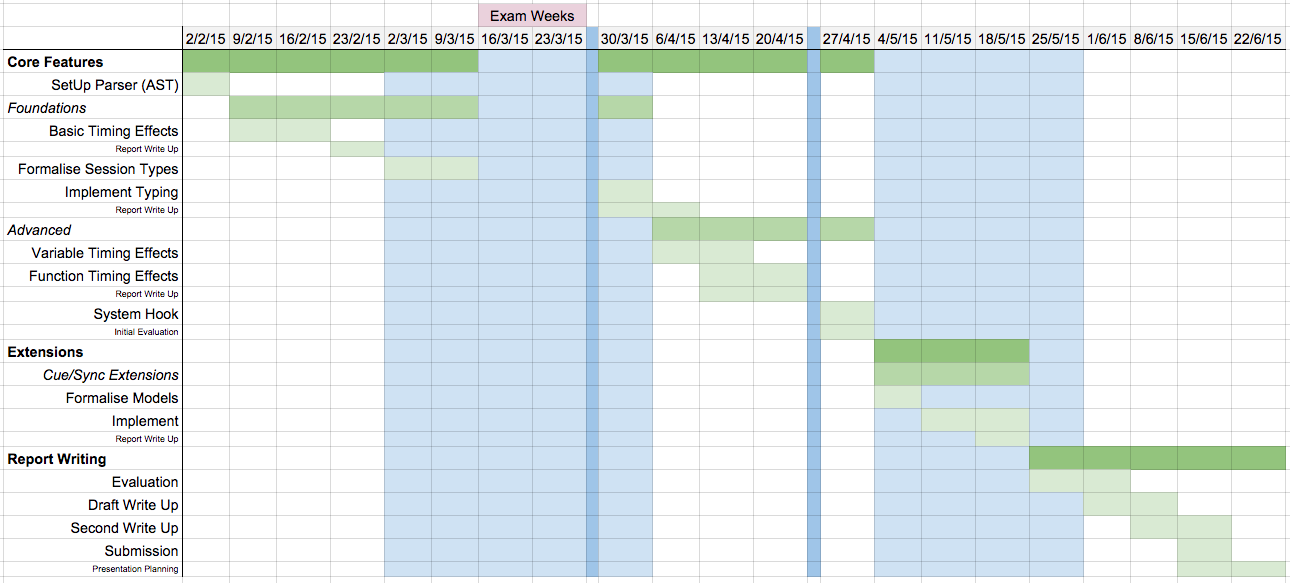
\includegraphics[width=\textwidth]{images/gantt-two.png}
\end{figure}

The weeks of the 16\textsuperscript{th} and 23\textsuperscript{th} of March are reserved for revision and
exam times. Before this work load is spread with consideration for courseworks
and after this most of the time is allocated with project work in mind. Core
requirements are aimed to be completed by the end of the Easter break. The weeks 
after that can be used as contingency in the case of unforseen circumstances, or
for some extension work as suggested below.

\begin{itemize}
	\item SetUp Parser: The bulk of the work cannot be completed without a good 
	representation of the AST of the language. Some time will be spent finding 
	one that is easy to use and descriptive.
	\item Timing Effects Features: The aim will be for the program to parse a 
	Sonic Pi code piece provided to it and be able to calculate the virtual time 
	of the program at each stage. The implementation is broken into different 
	steps, Constant Timing being the parsing of simple constant expression, 
	Variable Timing and Function Timing being those more complex timing elements 
	where variables are passed to different functions in the code or when the 
	timing is dynamically calculated.
	\item Formalise Session Types: The current form of Sonic Pi does not have a 
	full description of the application of session types to the language. The 
	focus on this will be extending the existing formulisation to include local 
	branching, recursion and delegation of session types in Sonic Pi.
	\item Implementing Types: This continues the previous point, the idea being 
	to physically implement the features within the language. This will also act 
	as tests that the formalisation is written well enough.
	\item System Hook: Run the verification within the real Sonic Pi IDE
	\item Cue/Sync Extensions: Currently the cue and sync primitives are very 
	simplistic, they have no ability to choose what to send and receive in their 
	messages. This extension will look into building on these primitives and 
	consider channel passing within session types. There is time allocated for 
	formalising the initial ideas and then implementing these into the language.
\end{itemize}

All items have been allocated some time to write up information about the tasks 
completed, both in terms of report details and any evaluation data presented. 
This will ensure maximum utilisation of the time allocated for reporting at the 
end of the project. Report Submission is dated for the week of the 15
\textsuperscript{th} of June. Presentation planning will overlap with this final 
week of reporting as presentations will be given the following week.

\subsection{Evaluation Outline}
As this is an educational program it would be ideal if some evaluation would 
take the form of user studies of Sonic Pi and the extensions made in this 
project. User groups could contain both those who have used the system before 
and those who have not, split equally between those who have a technical 
background and those who have none. It would be interesting to note whether 
any of those in the User Groups maintained any other creative hobbies outside 
of this field and how many had some kind of musical awareness and relate this 
to their reports and the overall findings of the tests.

Another piece that would be of interest would be discovering the execution 
times of the project on the different architectures that are available. Part 
of the objectives of the project is to provide a small verification system to 
run in parallel with a currently running program thread. For this to be a 
viable addition it must be fast and efficient enough not to interrupt with the 
existing functionality. On the Windows and Mac versions of the system it is 
unlikely to make much impact but the Raspberry Pi system is much smaller in 
it's capabilities.

% \section{Final Thoughts}

\begin{thebibliography}{9}

\bibitem{naec}
  \emph{http://www.naec.org.uk/events}

\bibitem{sp}
  \emph{http://sonic-pi.net/}

\bibitem{rp}
  \emph{http://www.raspberrypi.org/about/}

\bibitem{AB13}
  Aaron, S. and Blackwell, A.F.,
  \emph{From Sonic Pi to Overtone: Creative Musical Experiences with Domain-Specific and Functional Languages},
  The First ACM SIGPLAN Workshop on Functional Art, Music, Modeling \& Design,
  Boston, Massachusetts, USA,
  ACM, pp. 35-46,
  (2013)

\bibitem{AOB14}
  Aaron, S., Orchard, D. and Blackwell, A.F.,
  \emph{Temporal Semanics for a Living Coding Language},
  Proceedings of the 2nd ACM SIGPLAN International Workshop on Functional Art, Music, Modeling \& Design,
  Boston, Massachusetts, USA,
  ACM, pp. 37-47,
  (2014)

\bibitem{BAD14}
  Blackwell, A.F., Aaron, S. and Drury, R., 
  \emph{Exploring Creative Learning for the Internet of Things Era},
  In B. du Boulay and J. Good (Eds) Proceedings of the Psychology of Programming Interest Group Annual Conference, 
  pp. 147-158,
  (PPIG 2014)

\bibitem{BC05}
  Blackwell, A.F. and Collins, N.,
  \emph{The Programming Language as a Musical Instrument},
  In Proceedings of the Psychology of Programming Interest Group Annual Conference,
  pp. 120-130,
  (PPIG 2005)

\bibitem{BMNR14}
  Blackwell, A., McLean, A., Noble, J. and Rohrhuber, J.,
  \emph{Collaboration and Learning Through Live Coding},
  Dagsthul Seminar, Dagstuhl Reports 3,
  no. 9, pp. 130-168,
  (2014)

\bibitem{Ch12}
  Church, L., Rothwell, N., Downie, M., deLahunta, S. and Blackwell, A.F.,
  \emph{Sketching by Programming in the Choreohraphic Language Agent},
  In Proceedings of the Psychology of Programming Interest Group Annual Conference,
  pp. 163-174,
  (PPIG 2012)

\bibitem{DfEO13}
  Department for Education and Ofsted,
  \emph{ICT in schools: 2008 to 2011},
  Piccadilly Gate,
  Manchester,
  110134,
  (2013)

\bibitem{DfE13}
  Department for Education,
  \emph{National curriculum in England: computing programmes of study (key stages 1 - 4)},
  (2013)

\bibitem{HJ94}
  Hansson, H. and Jonsson, B.,
  \emph{A Logic for Reasoning About Time and Reliability},
  Formal Aspects of Computing 9,
  no 5., pp. 512-535,
  (1994)

\bibitem{HMBCY11}
  Honda, K., Mukhamedov, A., Brown, G., Chen, T. and Yoshida, N.,
  \emph{Scribbling Interactions with a Formal Foundation},
  In 7th International Conference on Distributed Computing and Internet Technology,
  p. 55 - 75,
  (ICDCIT 2011)

\bibitem{HVM98}
  Honda, K., Vasconcelos, V.T. and Kubo, M.,
  \emph{Language Primitives and Type Disciplines for Structured Communication-Based Programming},
  ESOP'98, LNCS 1381,
  pp. 22-38,
  (1998)

\bibitem{IG13}
  The IEEE and The Open Group,
  \emph{Sleep - The Open Group Base Specifications Issue 7, 2013},
  http://pubs.opengroup.org/onlinepubs/9699919799/functions/sleep.html,
  Retrieved 15 May,
  (2014)

\bibitem{McD07}
  McDirmid, S.,
  \emph{Living it Up with a Live Programming Language},
  Proceedings of the 22Nd Annual ACM SIGPLAN Conference on Object-oriented Programming Systems and Applications,
  New York, USA,
  ACM, pp. 623-638
  (2007)

\bibitem{McL13}
  McLean, A.,
  \emph{The Textual X},
  Proceedings of xCoAx2013: Computation Communication Aesthetics and X,
  pp. 81-88,
  (2013)

\bibitem{ME14}
  McDirmid, S. and Edwards, J.,
  \emph{Programming with Managed Time},
  Tech. Report, Microsoft,
  (2014)

\bibitem{NY14}
  Ng, N. and Yoshida, N.,
  \emph{Pabble: Parameterised Scribble for Parallel Programming},
  In 22nd Euromicro International Conference on Parallel, Distributed and Network-Based Processing, 
  p. 707 - 714,
  (PDP 2014)

\bibitem{LDW87}
  Lee, I., Davidson, S. and Wolfe, V.,
  \emph{Motivating Time as a First Class Entity},
  Technical Reports (CIS),
  pp. 288,
  (1987)

\bibitem{SG10}
  Sorensen, A. and Gardner, H.,
  \emph{Programming with Time: Cyber-Physical Programming with Impromptu},
  ACM Sigplan Notcies 45,
  no. 10, 822-834,
  (2010)

\bibitem{W10}
  Woolford, K., Blackwell, A.F., Norman, S.J. \& Chevalier, C.,
  \emph{Crafting a Critical Technical Practice},
  Leonardo 43(2),
  202-203,
  (2010)

\bibitem{WC03}
  Wang, G. and Cook, P.R.,
  \emph{ChucK: A Concurrent, On-The-Fly Audo Programming Language},
  International Computer Music Conference,
  pp. 1-8,
  (2003)

\bibitem{Wing06}
  Wing, J.M.,
  \emph{Computational Thinking},
  Communication of the ACM,
  Vol. 49, pp. 33-35,
  (2006)

\end{thebibliography}

\end{document}